\chapter*{London}

In 1948 ben ik naar Londen vertrokken, ik was toen 20. In de oorlog kon je niks. En toen las ik eens een keer iets over Londen. En toen dacht ik. Als het weer vrede is dan wil ik naar Londen! Dat leek me zo enig! 

Een poos daarvoor heeft een meisje uit Londen bij ons een uitwisseling gedaan. Ze is toen veertien dagen blijven logeren. Via haar heb ik destijds het adres van een gezin in Walton on Thames gekregen. 

Dit meisje, een kraamverzorgster, heeft daar nog een goed woordje voor me gedaan. Ik weet alleen niet meer hoe ze heette. Na een briefwisseling mocht ik bij het gezin aan de slag als hulp in de huishouding. 

Mijn doel was om mijn Engels te verbeteren. Voordat ik naar Londen ging was mijn Engels al best goed. Maar toch wilde ik graag nog beter worden zodat ik het wat makkelijker zou kunnen spreken. Jaa, want ik wilde in eerste instantie eigenlijk stewardess worden! Maar helaas is dat nooit gebeurd hoor. Haha. 

\begin{figure}[h]
    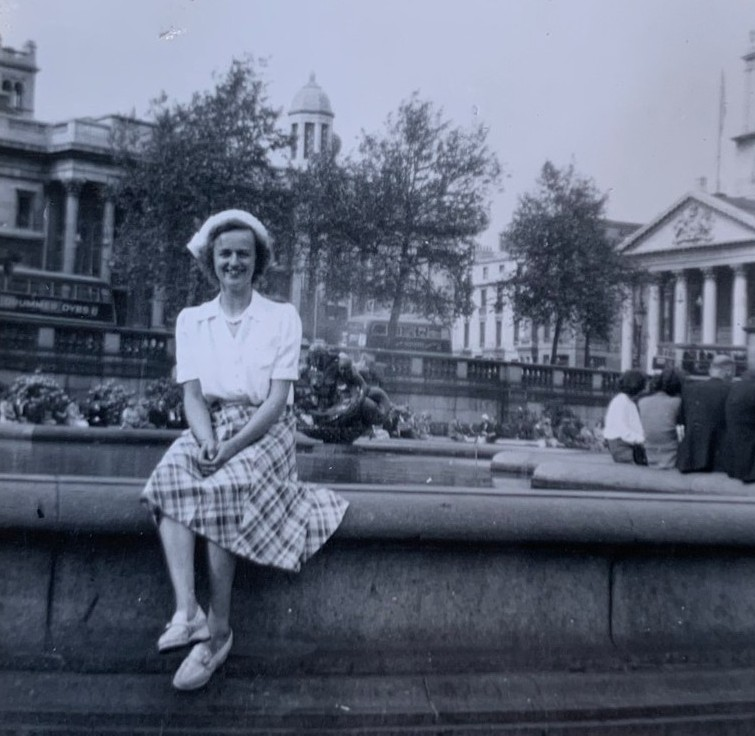
\includegraphics[width=\textwidth]{image28}
    \caption{Op Trafalgar square.}
\end{figure}

Dit was mijn eerste grote reis. In de oorlog mocht je namelijk het land helemaal niet uit.

Mijn vader en moeder lieten het door de vingers dat ik zo ver van huis wilde. ‘’Als je dit echt wil, zullen wij je niet tegenhouden’’ zeiden ze. Ze vonden het best. 

Voor ik naar London ging had ik al een foto gezien van Trafalgar square. Ik vond dat echt London! En ik had toen al bedacht dat ik daar op de foto wou.

Mijn broer Kees heeft me destijds naar de boot gebracht in Hoek van Holland. Vroeg in de ochtend gingen we samen met de trein. Maar eenmaal bij de douane mocht ik de boot helemaal niet op. Ik werd tegengehouden omdat ik geen werkvergunning had. Dit wist ik of het gezin waar ik zou komen te werken van tevoren helemaal niet. 

Het was een hele bedoening en de politie kwam er zelfs bij. Een vriendelijke Nederlandse jongen schoot me te hulp en na heel wat telefoontjes, tevergeefs vertrok de boot uiteindelijk zonder mij. Dus kon ik weer terug naar huis!

Na een lange reis kwam ik s’ avonds laat weer thuis aan. Het was al lang donker toen ik op de deur klopte. Mijn vader deed de deur open: ‘’Dag mevrouw’’ zei mijn vader. Want hij herkende me helemaal niet. Ik zei: ‘’Hallooo, hier ben ik weer!’’ Ik had ze van te voren niet gebeld, want dan zouden ze zich daar alleen maar druk over maken. 

Na een briefwisseling met het gezin uit ‘Walton on Thames’, bellen met Engeland dat was veel te duur, was een werkvergunning alsnog zo geregeld en kon ik de keer daarna zo de douane door.  

Na aankomst in Engeland werd ik door de heer des huizes ‘Gerald Wilson’ opgehaald. Eerst gingen we naar het politiebureau om de ‘working permit’ te checken. Dat moest toen nog.

Gerald Wilson, werkte oorspronkelijk bij de marine, in een basis in Hong Kong, hij is toen gevangengenomen door de Japanners en in een concentratiekamp terechtgekomen. Gelukkig heeft hij het overleefd en na de oorlog werkte hij als ingenieur. Hij moest toen niets meer te maken hebben met alles wat maar uit Japan kwam.

De vrouw heette: Dorothy (Kitching?) Toen ik daar aan kwam hadden ze twee meisjes. Jillian en Judith. Jillian was de oudste. Aan het einde van het jaar dat ik er was bleek Dorothy in verwachting van een derde kind. Dit werd een jongetje. (John) En daarna toen ik weer terug in Nederland was hebben ze nog een zoon gekregen. (Charles).

De band met de kinderen was destijds best! Alleen op een korte briefwisseling na hebben we eigenlijk geen contact meer gehouden. 

Ze woonden in een heel mooi vrijstaand huis met een grote tuin er omheen. Ashley Park Avenue, dat was het adres. Het huisnummer weet ik niet meer. Ze hadden ook nog kippen. Want ja voedsel was schaars en dat was toen zelfs nog op de bon. 

Ook kreeg ik Engelse les. Voor het eindexamen moesten we een essay schrijven. Als onderwerp koos ik de bezetting. Ik had het een beetje aangedikt. Toen hebben ze mijn essay eruit gepikt en het voorgedragen in de klas! Alleen heb ik dat zelf gemist omdat ik toen op een afspraak was. 

\begin{figure}[h]
    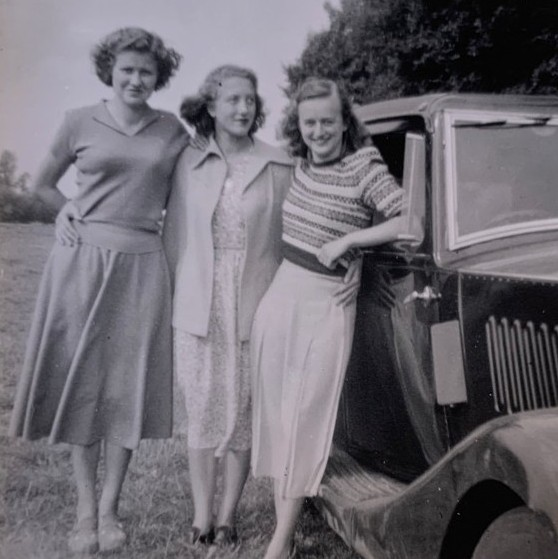
\includegraphics[width=\textwidth]{image29}
    \caption{Hollandse vriendinnen.}
\end{figure}

Ik had \'{e}\'{e}n dag in de week vrij. Dan ging ik meestal op stap. Naar Londen Bijvoorbeeld. Met de trein. Ik ben \'{e}\'{e}n keer zelfs helemaal naar de zuidkust gegaan! Dat was prachtig. 

In mijn tijd in Walton on Thames heb ik een paar andere Nederlandse meisjes ontmoet. Daar was het wel leuk mee, alleen thuis zouden het niet mijn vriendinnen geweest zijn. 

Er waren geen leuke jongens. Daar had ik eigenlijk ook helemaal geen behoefte aan. En tja, dat is zo lastig een lange afstandsrelatie met een man uit Engeland. 

Er waren in de buurt een keer een stel Hollandse voetballers op bezoek. Toen kreeg ik een uitnodiging voor een ‘gezellige avond’. Daar had ik helemaal geen zin in! Haha. Ik ben wel ooit een leuke Amerikaanse jongen op de fiets tegengekomen. Maar dat was uiteindelijk toch ook niks.

Het gezin was heel prettig. Het waren beschaafde en bescheiden mensen. Ik hoorde van de andere Nederlandse meisjes die daar ook werkten dat dat soms wel anders was. Dan moesten ze een bejaarde vrouw verzorgen bijvoorbeeld, en ja dan ontmoette je verder ook niemand! 

Ik moest in het huishouden ook koken. Uitdaging was dat ik daar ineens Engels moest koken. Op een dag kwam de heer des huizes naar beneden om een compliment te geven over het uitstekende eten. Nou dat was heel wat! 

Opvallend vond ik dat wanneer ‘de heer des huizes’ thuiskwam van werk hij steevast mopperde over dat de mensen zo weinig met elkaar praatten in de trein. Dan zaten er elke dag dezelfde mensen in de trein, maar niemand deed zijn mond open! Dat vond hij verschrikkelijk. Maar zo zijn ze. De Engelsen. 

Het leukste vond ik dat ik opgegeven moment in het Engels droomde. Dat kwam omdat je het natuurlijk de hele dag sprak, en ja dan droomde ik ineens in het Engels! 

Na een tijdje in Engeland te hebben gewoond was mijn Engels dan ook ‘’ontzettend goed’’ 

\begin{figure}[h]
    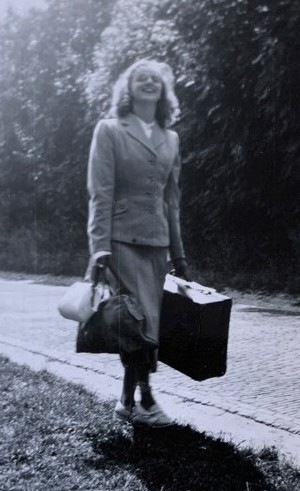
\includegraphics[width=.9\textwidth]{image30}
    \caption{op vakantie naar Holland.}
\end{figure}

Het grootste compliment wat ik kreeg kwam van een dame van de winkel waar ik een jasje aan het passen was. Ik zei tegen de mevrouw die me aan het helpen was: ‘dit jasje vind ik niet zo leuk’. Waarop de dame van de winkel antwoorde: ‘’Oh, die lijkt natuurlijk een beetje op wat u op de kostschool gedragen heeft!’’ En ik heb natuurlijk nooit op de kostschool in Engeland gezeten. 

Ik heb het ontzettend naar mijn zin gehad. Maar Nederland was mijn thuis. Mijn ouders en familie waren er nog. En ja daar wilde ik natuurlijk wel een beetje bij in de buurt zijn. Ik wilde eigenlijk maar een jaar blijven.

Maar op een dag kwam de vrouw des huizes naar me toe en zei: ‘’Och Tine, zou je alsjeblieft nog even willen blijven? Ik ben namelijk weer in verwachting’’ En toen ben ik nog een half jaartje langer gebleven. En dat vond ik wel genoeg. Ik had mijn doel bereikt. 

Na terugkomst uit Londen ben ik eigenlijk gelijk aan het werk gegaan. En ben ik terecht gekomen in Huis ter heide. 

Wil je nog meer weten over Londen?? Nah, nou is het klaar hoor! Haha (Einde interview).